\documentclass[10pt,xcolor={svgnames}]{beamer}
%\usefonttheme[onlymath]{serif}
%%%%% Colors
\usetheme{Dresden}%\usetheme{Madrid}
\colorlet{beamer@blendedblue}{green!55!black}
%%%%%

%%%%% Other 
\beamertemplatenavigationsymbolsempty
\addtobeamertemplate{navigation symbols}{}{%
	\usebeamerfont{footline}%
	\usebeamercolor[fg]{footline}%
	\hspace{1em}%
	\insertframenumber/\inserttotalframenumber
}
\usepackage{hyperref, url}
%\usepackage[symbol]{footmisc}

\definecolor{pine_green}{HTML}{007935}
\hypersetup{colorlinks,breaklinks,linkcolor=white,urlcolor=orange,citecolor=black}
\renewcommand\thefootnote{\textcolor{pine_green}{\arabic{footnote}}}
\setbeamercolor{alerted text}{fg=pine_green}

\renewcommand{\i}{\mathnormal{I}}

\usepackage{cancel}
\usepackage{ulem}
\usepackage{multirow}
\usepackage{mathtools}
%% Note that makecell calls array, so it is incompatile with sgame
%\usepackage{makecell} 
\usepackage{multicol}
\usepackage{tikz}
\newcommand{\tr}[1]{\textcolor{red}{#1}}
\DeclarePairedDelimiter{\abs}{\lvert}{\rvert}
\renewcommand{\epsilon}{\varepsilon}
\setbeamertemplate{itemize subitem}{\textbullet}
\setbeamertemplate{itemize subsubitem}{$\circ$}

%https://tex.stackexchange.com/questions/289542/auto-resizing-parenthesis-in-math-formulas
% \usepackage{amsmath} for testing
\newcommand*\autoop{\left(}
\newcommand*\autocp{\right)}
\newcommand*\autoob{\left[}
\newcommand*\autocb{\right]}
\AtBeginDocument {%
	\mathcode`( 32768
	\mathcode`) 32768
	\mathcode`[ 32768
	\mathcode`] 32768
	\begingroup
	\lccode`\~`(
	\lowercase{%
		\endgroup
		\let~\autoop
	}\begingroup
	\lccode`\~`)
	\lowercase{%
		\endgroup
		\let~\autocp
	}\begingroup
	\lccode`\~`[
	\lowercase{%
		\endgroup
		\let~\autoob
	}\begingroup
	\lccode`\~`]
	\lowercase{%
		\endgroup
		\let~\autocb
}}

\delimiterfactor 1001

\makeatletter
% for amsmath "compatibility" (not sophisticated)
% \usepackage{amsmath}
\AtBeginDocument {%
	\def\resetMathstrut@{%
		\setbox\z@\hbox{\the\textfont\symoperators\char40}%
		\ht\Mathstrutbox@\ht\z@ \dp\Mathstrutbox@\dp\z@}%
}%
\makeatother
%%%%%

%%%%% Greying out/invisible Slides
%\setbeamercovered{invisible}
%\setbeamercovered{%
	%  again covered={\opaqueness<1->{15}}}

%%%%%







%%%%% Footnotes and captions
%\usepackage[utf8]{inputenc}
\usepackage{caption}
\usepackage{comment}
\setbeamerfont{footnote}{size=\tiny}
\setbeamerfont{caption}{size=\small}
%\setbeamerfont{normal text}{size=\small}
\setbeamerfont{itemize/enumerate body}{size=\small}
\setbeamerfont{itemize/enumerate subbody}{size=\footnotesize}
%%%%%


%%%%
\usepackage{booktabs}
\usepackage{multirow,bigstrut}
%\usepackage{tabu}
\graphicspath{{C:/Users/gamec/Documents/School/EC 201 Fa21}​​}
\usepackage{pstricks}
%\usepackage{pstricks, pst-node}
\usepackage{sgamevar}
%%%%



%Information to be included in the title page:
\title[Connor Wiegand]{Intro to Economic Analysis: Microeconomics}
\subtitle{EC 201 - Day 20 Slides}
\author[EC 201]{Connor Wiegand}
\institute[]{Department of Economics - University of Oregon}
\date{1 December 2021}


\begin{document}

\frame{\titlepage}

\section*{Intro to Game Theory}

\begin{frame}{Logistics}
	\begin{itemize}
		\item Homework 8 due \underline{this} Monday (Monday of finals week, Dec 6th at 11:59pm)
		\item Comprehensive final exam on \underline{December 9th} at 2:45pm -- the exam will last for 2 hours
	\end{itemize}
\end{frame}


\begin{frame}{Dictator Game}
	\begin{itemize}[<+->]
		\item Pair up: Youngest is dictator, eldest is acceptor
		\item The dictator has $\$100$, and can choose an offer amount $\$x$, that the other player receives out of their $\$100$
		\item The acceptor is allowed to reply to the offer with ``yes" or ``no"
		\begin{itemize}
			\item If yes, both players keep their money
			\item If no, both players get nothing
		\end{itemize}
		\item Play
		\item Switch
		\item What should you do?
		\begin{itemize}
			\item If you are just playing once and you value money, offer $\$0$/ always accept (unless maybe the offer is literally $\$0$, in which case it doesn't matter)
			\item What actually happens? Do people care about spite? How does this change if people are expecting another round?
		\end{itemize}
	\end{itemize}
\end{frame}


\begin{frame}{What is a Game?}
	\begin{itemize}[<+->]
		\item Loose definition: a game consists of (i) players, (ii) strategies (also called \textit{moves}, or \textit{actions}), and (iii) payoffs
		\item This is a very broad definition, and allows for a lot of different things to count as games
		\begin{itemize}
			\item It is also one of the test questions I can ask you 
		\end{itemize}
		\item Strategery is important, because interactive elements are what make games interesting
		\begin{itemize}
			\item For instance, a bunch of people separately making decisions is more accurately described as \textit{decision theory}
		\end{itemize}
		\item What are some games that you have heard of, or can think of?\vspace{-3mm}
		\begin{multicols}{2}
			\begin{itemize}
				\item Duopoly -- two firms picking prices or quantities
				\item Prisoner's Dilemma
				\item Matching Pennies
				\item Battle of the Sexes
				\item Quiche/Beer
				\item Dictator game
				\item 2/3 of average
				\item Centipede Game
				\item Chicken
				\item Rock, Paper, Scissors
				\item Signaling Game
			\end{itemize}
		\end{multicols}
	\end{itemize}
\end{frame}

\begin{frame}{Who Cares about Game Theory?}
	\begin{itemize}[<+->]
		\item There are other games, too: Chess, League of Legends, Poker, etc. 
		\item Game theory is the careful analysis of interactive games, and what makes these game interesting is their true complexity
		\item Game theory cannot make you win a League match\footnote{``The only winning move is not to play."- \textit{WarGames} (1983)}, but it \textit{can} help you analyze specific decisions that come in such complex games
		\item Who cares about game theory?
		\begin{itemize}
			\item Coke/Pepsi (or other duopolies)
			\item Amazon
			\item Verizon
			\item Game Studios? 
		\end{itemize}
	\end{itemize}
\end{frame}

\begin{frame}{Everyday Uses}
	\begin{itemize}[<+->]
		\item Much like intuition in this class helps you understand why things happen in the real world, game theory can also help with understanding the optimal/best ways to make interactive decisions:
		\vspace{-2mm}
		\begin{multicols}{2}
			\begin{itemize}
				\item When should I email my professor to ask for a favor?
				\item When and how should I reveal my valuation when buying a car?
				\item When my annoying family member says something during th holidays, should I provide a legitimate counterargument, or just gaslight them?
				\item How should I interact with this business on a regular basis in order to minimize costs, and keep me from getting screwed over? 

				\item Should I buy my my girlfriend new boobs?\footnote{If anyone is reading this, this isn't my example}
				\item What happens if your wife gets kidnapped? (Don't use game theory)
			\end{itemize}
		\end{multicols}
	\end{itemize}
\end{frame}


\begin{frame}{2/3 Average}
	\begin{itemize}[<+->]
		\item Everyone write down a number between 0 and 100, inclusive ($[0,100]$). You win if you correctly guess 2/3 of the average of everyone's score (we will call $\frac{2}{3}$ of the average the ``target score"). 
		\item What's your guess?
		\item What's the best strategy?
	\end{itemize}
\end{frame}

\begin{frame}{2/3 Average Solution}
	\begin{itemize}[<+->]
		\item Note: the maximum that anyone can say is 100. If everyone said 100, the average would be 100, so $2/3$ of the average would be $66.\bar{6}$, so this is the largest target score
		\begin{itemize}
			\item Thus, it is extremely unlikely that anyone would play 66.6-100, so we can effectively eliminate those strategies when trying to guess the average
			\item If the only reasonable guess is less than or equal to 66.6, then the maximum reasonable average is 66.6
			\begin{itemize}
			\item This makes the largest reasonable target score $\frac{2}{3}(66.6)=44.4$
			\item So now, the largest reasonable guess is 44.4
			\item But this will make the largest reasonable target score 29.629
			\end{itemize}
		\end{itemize}
		\item As we keep repeating this thinking, what happens?
		\item The only guess that is left is \underline{\textit{zero}}
		\item Is this what we see?
		\begin{itemize}
			\item A Danish newspaper tried this with about 19,000 respondents, and the target number was found to be 21.6
			\item Even among economists, no
		\end{itemize}
	\end{itemize}
\end{frame}

\begin{frame}{The Rules of the Game}
	\begin{itemize}[<+->]
		\item Today, we will mostly talk about games with 2 players and 2 strategies
		\item Players only play once, and they do not communicate before or during the game
		\item If our players are named $A$ and $B$, the following is true:
		\begin{itemize}
			\item $A$ knows how to play the game, and B knows how to play the game
			\item $A$ knows that $B$ knows how to play the game, and $B$ knows that $A$ knows how to play the game
			\item $A$ knows that $B$ knows that $A$ knows how to play the game, and $B$ knows that $A$ knows that $B$ knows how to play the game
			\item ...So on and so forth
			\item This seems silly, but game theorists have spent a great deal of time analyzing what happens when the $n^{\text{th}}$ iteration of this thinking fails
			\begin{itemize}
				\item Here is an interesting application of this principle \href{https://youtu.be/98TQv5IAtY8}{Green-Eyed Islander Puzzle}
			\end{itemize}
		\end{itemize}
	\end{itemize}
\end{frame}

\begin{frame}{Normal Form Games}
	\begin{itemize}[<+->]
		\item If these (and some other, subtler principles) are satisfied, we may write down what's called a \underline{Normal Form Game}\footnote{Note: this isn't the only way to represent a game}
		\begin{figure}
			\begin{game}{2}{2}[$P_{A}$][$P_{B}$]
				\> $L$      \> $R$\\
				$U$   \> $a,b$  \> $c,d$\\
				$D$   \> $e,f$   \> $g,h$
			\end{game}
			\hspace{5mm} or \hspace{5mm}
			\begin{game}{2}{2}[$P_{A}$][$P_{B}$]
				\> $L$      \> $R$\\
				$U$   \> $\pi^{A}_{11},\pi^{B}_{11}$  \> $\pi^{A}_{12},\pi^{B}_{12}$\\
				$D$   \> $\pi^{A}_{21},\pi^{B}_{21}$   \> $\pi^{A}_{22},\pi^{B}_{22}$
			\end{game}
		\end{figure}
		\item Player $A$ ($P_{A}$) can play Top or Bottom, while player $B$ can play Left or Right
		\item The first entry in each cell denotes player $A$'s payoff if each player plays the corresponding move, while the second entry represents $B$'s payoff
		\begin{itemize}
			\item For instance, if $A$ plays Top and $B$ plays Left, then player $A$ receives $a$ (or $\pi^{A}_{11}$), while $B$ receives $b$ (or $\pi^{B}_{11}$)
		\end{itemize}
		\item Players are trying to maximize their utility 
	\end{itemize}
\end{frame}

\section*{Analyzing Games}

\begin{frame}{The Most Famous Game}
	\begin{itemize}[<+->]
		\item In game theory, the most popular (and probably mostly richly studied) is the prisoners dilemma
		\item Story: Ariana and Byron get caught trying to steal cars at a car wash
		\item Ariana and Byron both are being separately interrogated by the police
		\begin{itemize}
			\item If neither snitches, they both go to jail for 5 years, because the police can't prove anything
			\item If Araiana snitches on Byron, but Byron keeps quiet, then Ariana gets off scot-free, but Byron goes away for 20 years (and vice versa)
			\item If both players snitch, then both go away for 10 years
		\end{itemize}
			\item Here is the game in Normal Form:
			\begin{center}
				\begin{game}{2}{2}[$A$][$B$]
					\> $Q$      \> $S$\\
					$Q$   \> $-5,-5$  \> $-20,0$\\
					$S$   \> $0,-20$   \> $-10,-10$
				\end{game}
			\end{center}
	\end{itemize}
\end{frame}

\begin{frame}{Example Prisoner's Dilemma}
	\begin{itemize}[<+->]
		\item Again, here is the game we are considering:
		\begin{center}
			\begin{game}{2}{2}[$A$][$B$]
				\> $Q$      \> $S$\\
				$Q$   \> $-5,-5$  \> $-20,0$\\
				$S$   \> $0,-20$   \> $-10, -10$
			\end{game}
		\end{center}
		\item What do you think happens?
		\begin{itemize}
			\item In theory and \underline{very} often in practice, both players snitch
		\end{itemize}
		\item Okay, but how do talk about this economically?
		\item Much like the 2/3 average game, we do so by iteratively thinking about what a \textit{rational} person would do 
		\begin{itemize}
			\item Much of game theory is about assuming the other player is rational, narrowing down their rational decisions, and then seeing what another player would do, given what is rational for the first player
		\end{itemize}
	\end{itemize}
\end{frame}

\begin{frame}{Analyzing Prisoner's Dilemma}
	\begin{itemize}[<+->]
		\item Remember, the players cannot talk before or while the game \vspace{-3mm}
		\begin{center}
			\begin{game}{2}{2}[$A$][$B$]
				\> $Q$      \> $S$\\
				$Q$   \> $-5,-5$  \> $-20,0$\\
				$S$   \> $0,-20$   \> $-10,-10$
			\end{game}
		\end{center}\vspace{1mm}
		\item Let's suppose we thought both players could keep quiet 
		\begin{itemize}
			\item Consider Ariana: she cannot control what Byron does, but she can control what she does
			\item If she were to ``switch" strategies\footnote{They are only playing once. By ``switch", I mean that we are thinking hypothetically. One might also say ``she might instead play"}, she would change her payoff from $-5$ to $0$, an improvement
		\end{itemize}
		\item So now let's consider $(S,Q)$ (Ariana plays $S$, Byron plays $Q$)
		\begin{itemize}
			\item Ariana now does not want to deviate from this strategy, so let's consider Byron
			\item Given that Byron is ``currently" playing $Q$, switching to $S$ will have a better payoff (-10 vs -20) for him
			\begin{itemize}
				\item That is, given that he knows (...) that playing $Q$ will mean Araiana plays $S$, he should play $S$
			\end{itemize}
		\end{itemize}
	\end{itemize}
\end{frame}

\begin{frame}{Analyzing Prisoner's Dilemma, (cont.)}
	\begin{itemize}[<+->]
		\item We could repeat that whole analysis starting with Byron instead of Ariana \vspace{-3mm}
		\begin{center}
			\begin{game}{2}{2}[$A$][$B$]
				\> $Q$      \> $S$\\
				$Q$   \> $-5,-5$  \> $-20,0$\\
				$S$   \> $0,-20$   \> $-10,-10$
			\end{game}
		\end{center}\vspace{1mm}
		\item Also note that starting at $(Q,S)$ or $(S,Q)$ resumes the above argument in the middle, and still leads us to $(S,S)$
		\item What happens when we consider $(S,S)$ as a possible outcome?
		\begin{itemize}
			\item Remember, players can't explicitly coordinate
			\item Does any of them have any incentive to \underline{individually} deviate from this spot?\vspace{-3mm}
			\begin{itemize}
				\item \textit{No.}
			\end{itemize} 
		\end{itemize} 
		\item This last point is important to defining why $(S,S)$ is something worth calling an ``equilibrium", and summing up this whole argument
		\item For the test, I want to be able to give you a prisoner's dilemma (with possibly varied notation), and show that you know that both players snitching is the solution
	\end{itemize}
\end{frame}




\begin{frame}{Nash Equilibrium (NE)}
	\begin{itemize}[<+->]
		\item In game theory, the thing we call a ``solution" or ``equilibrium" to a game is called a \underline{\textit{Nash Equilibrium}}
		\item To define it formally, we need the notion of a \textit{best response}
		\item A \underline{\textbf{Best Response}} is the strategy (or strategies) which produces the most favorable outcome for a player, taking other players' strategies as given
		\begin{itemize}
			\item Symbolically, given other players' strategies $S$ as given, my payoff of playing $s$ is better than (or at least as good as) any other strategy $s'$, given $S$:
			$$\pi^{i}(s|S)\ge \pi^{i}(s'|S)$$
		\end{itemize}
		\item Definition: A \underline{\textbf{Nash Equilibrium}} is a set of mutually best responses
		\begin{itemize}
			\item In short, a Nash Equilibrium is ``a set of strategies such that no player has the incentive to unilaterally (individually) deviate from their chosen strategy"
			\item For the test, I want you to know what a Nash Equilibirum is
		\end{itemize}
	\end{itemize}
\end{frame}

\begin{frame}{How Do We Find Nash Equilibria?}
	\begin{itemize}[<+->]
		\item This just describes the algorithm that we did to find the NE of Prisoner's Dilemma:
		\begin{enumerate}
			\item Given a normal-form game, start at a cell
			\item For each player, underline the best response
			\item Move to the next cell
			\item Repeat until done
		\end{enumerate}
		\item Here it is with PD:
		\only<6>{
		\begin{center}
			\begin{game}{2}{2}[$A$][$B$]
				\> $Q$      \> $S$\\
				$Q$   \> $-5,-5$  \> $-20,0$\\
				$S$   \> $0,-20$   \> $-10,-10$
			\end{game}
		\end{center}}
		\only<7>{
		\begin{center}
			\begin{game}{2}{2}[$A$][$B$]
				\> $Q$      \> $S$\\
				$Q$   \> $-5,-5$  \> $-20,\underline{0}$\\
				$S$   \> $\underline{0},-20$   \> $-\underline{10},-\underline{10}$
			\end{game}
		\end{center}} 
	\end{itemize}
\end{frame}


\begin{frame}{A Bigger Prisoner's Dilemma}
	\begin{itemize}[<+->]
		\item Recognize the following? It's just a prisoner's dilemma
		\begin{figure}
			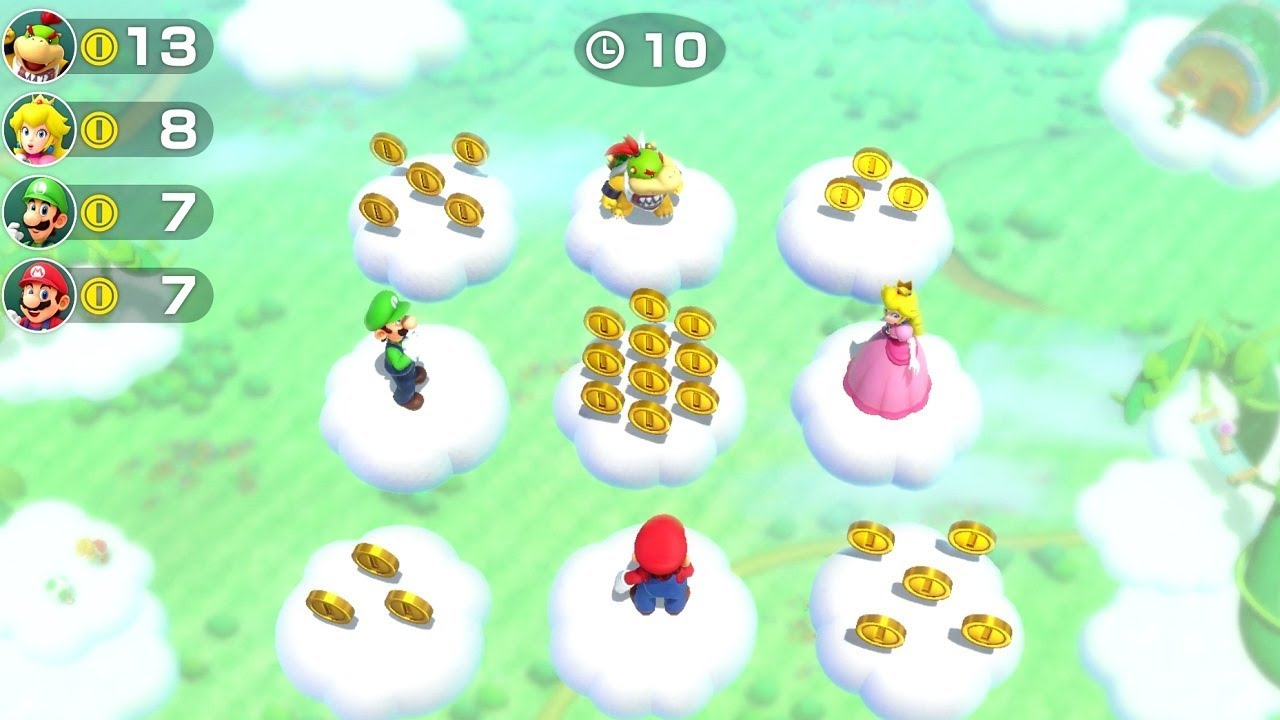
\includegraphics[width=9cm]{air to a fortune.png}
			\caption*{\textit{Air To A Fortune}, Mario Party Franchise}
		\end{figure}
	\end{itemize}
\end{frame}


\section*{Other Games}

\begin{frame}{Chicken}
	\begin{itemize}[<+->]
		\item Yes, that chicken: car who can stay or dodge, driving at a person who can stay or dodge 
		\begin{center}
			\begin{game}{2}{2}[Car][Pedestrian]
					\> $D$      \> $S$\\
				$D$   \> $-25,-25$  \> $-10, 40$\\
				$S$   \> $20, -5$   \> $-100,-\infty$
			\end{game}
		\end{center}
		\item We see two NE here: $(S,D)$ and $(D,S)$
		\begin{itemize}
			\item Either player wants to individually deviate from $(D,D)$, likewise with $(S,S)$
		\end{itemize} 
		\item Some questions to think about:
		\begin{itemize}
		\item How do we determine which is better?
		\item Do we think one will happen more often than the other?
		\item What happens if the car randomly plays $S$ half the time, and the pedestrian randomly plays $S$ one third of the time? What happens if we play with these probabilities?
	\end{itemize} 
	\end{itemize}
\end{frame}

\begin{frame}{BoS}
	\begin{itemize}[<+->]
		\item I want to go to the Bread Bank for dinner, but my girlfriend wants to eat at the Krusty Krab.
		\item Our phones died, so we just have to go to the restaurant individually and hope the other person is there
		\item We both value getting the food we want, as well as eating with the other person:
		\begin{center}
			\begin{game}{2}{2}[Me][Gf]
				\> KK      \> BB\\
				KK   \> $1,2$  \> $0,0$\\
				BB   \> $0,0$   \> $2,1$
			\end{game}
		\end{center}
		\item Again, we see two NE here, where we are both eating at the same restaurant
		\item What happens if each person plays KK with probability $2/3$?
		\item Suppose I have the option that morning to burn a dollar in front of my girlfriend, changing my payoffs by a dollar if I did. How would this change the outcome of the game?
	\end{itemize}
\end{frame}


\begin{frame}{Matching Pennies}
	\begin{itemize}[<+->]
		\item If the pennies match, I keep them. If not, you keep them:
		\begin{center}
			\begin{game}{2}{2}[Me][You]
				\> H      \> T\\
				H   \> $1,-1$  \> $-1,1$\\
				T   \> $-1,1$   \> $1,-1$
			\end{game}
		\end{center}
		\item This game has no NE that we can see
		\item The only solution is to randomize
		\begin{itemize}
			\item Fact: Every game with finite players and finite strategies has a solution
		\end{itemize}
	\end{itemize}
\end{frame}

\begin{frame}{Pascal's Wager}
	\begin{itemize}[<+->]
		\item Pascal: don't use this to believe in God, but if you are truly on the fence completely, here is a nifty argument:
		\begin{center}
			\begin{game}{2}{2}[You\Big|][\underline{Nature}]
					\> God Exists   \> God DNE\\
				Believe in God   \> $\infty$, ---  \> finite loss, --- \\
				Don't Believe in God  \> $-\infty$, ---   \> finite win, ---
			\end{game}
		\end{center}
		\item Solution: believe in God 
		\begin{itemize}
			\item Once again, even Pascal was not a huge fan of this as an argument
		\end{itemize}
		\item This isn't really a game, it's more of a decision
		\begin{itemize}
			\item Hopefully you can see that decisions can still be structured as games, they can still be interesting, but they lose their quintessential interactive flavor
		\end{itemize}
	\end{itemize}
\end{frame}


\begin{frame}{Repeated Games}
	\begin{itemize}[<+->]
		\item What happens if you play games more than once?
		\begin{itemize}
			\item Let's suppose that we know we will play PD infinitely many times
			\item Idea [Grim Trigger]: Start by cooperating; if you snitch once, I will play snitch every game thereafter for the rest of time
			\item Result: It's enough to incentivize cooperation forever
			\item Idea [Tit-for-Tat]: Copy your previous move
			\item Result: We will often either cooperate forever or swap forever
			\item There are variations of each of these
		\end{itemize}
		\item Can we commit to these things?
		\begin{itemize}
			\item What happens when you actually get down to having to punish the other player by snitching?
			\item What happens if you up-talk yourself before chicken?
			\item What happens if the other prisoner knows you will shoot them when you get out?
		\end{itemize}
	\end{itemize}
\end{frame}

\begin{frame}{Threats}
	\begin{itemize}[<+->]
		\item A threat may allow you to take a strategic move. But is it credible?
		\item You can say you absolutely won't dodge in chicken, but is it believable? Will you really die when it comes down to it?
		\item When analyzing games that have many steps, we often start from the end, and ask if people can make threats, and if those threats are credible enough to be taken seriously
		\begin{itemize}
			\item A credible threat is one that is costly, but not costly enough that you won't do it
		\end{itemize}
		\item JFK can threaten nuclear war in order to get missiles out of Cuba, but is that threat believable?\footnote{And should you really be threatening that?}
	\end{itemize}
\end{frame}


\begin{frame}{Tying Oneself to the Mast}
	\begin{itemize}[<+->]
		\item An interesting part of game theory is that restricting your choices can actually \textit{improve} your outcomes
		\begin{itemize}
			\item Ex: consider the game of chicken again. Suppose that I visibly step in a layer of quick dry cement. What will happen?
			\begin{center}
				\begin{game}{2}{2}[Car][Pedestrian]
					\> $D$      \> $S$\\
					$D$   \> $-25,-25$  \> $-10, 40$\\
					$S$   \> $20, -5$   \> $-100,-\infty$
				\end{game}
			\end{center}
		\item The driver will see that I cannot play $D$, so they are forced to choose between killing me and dodging, they will dodge 
		\end{itemize}
		\item Ulysses/Odysseus: tie me to the mast (and you all put wax in your ears), so that I can hear the song of the Sirens without jumping into the sea
		\item You may have done this when you \textit{asked} your mom to say no to your friend staying the night 
	\end{itemize}
\end{frame}





\begin{frame}{Summary}
	\begin{itemize}[<+->]
		\item Game theory is a whole discipline. It is hard to get through it all in one undergrad class, let alone a lecture. Hopefully I provided some thought-provoking intuition
		\item To summarize:
		\begin{itemize}
		\item A game consists of (i) players, (ii) strategies/actions/moves, and (iii) payoffs
		\item Much of game theory is about assuming the other player is rational, narrowing down their rational decisions, and then seeing what another player would do, given what is rational for the first player
		\item You can't do everything you want with game theory, but it is still very powerful
		\item A Nash Equilibrium is a set of mutual best responses, where no player will unilaterally deviate
		\item In a Prisoner's dilemma, both players will snitch in equilibrium
		\end{itemize}

	\end{itemize}
\end{frame}


\section*{Review}

\begin{frame}{}
	\begin{itemize}[<+->]
		\item 
	\end{itemize}
\end{frame}

\begin{frame}{Basic Overview of Topics (Pre-Midterm)}
	\begin{itemize}[<+->]
		\item The following list is a brief overview, and is by no means extensive
		\item PPF and OC (ch 1-3)
		\begin{itemize}
			\item Draw a PPF given production table, understand it's regions
			\item Shifting a PPF
			\item Compute OC from production table
			\item Combine two PPFs from trade 
		\end{itemize}
		\item Demand (/Supply) Curve (ch 4)
		\begin{itemize}
			\item How to draw one from data
			\item Individual curves $\to$ market curve
			\item What causes movement along, what shifts
			\item Law of demand (supply)
			\item Graphing with equations
		\end{itemize}
		\item Equilibrium (ch 4)
		\begin{itemize}
			\item Identifying, intuition behind markets
			\item Shifting both supply and demand, and seeing the impact on equilibrium $P$ and $Q$
			\item Graphing
		\end{itemize}
	\end{itemize}
\end{frame}

\begin{frame}{Basic Overview of Topics (Pre-Midterm)}
	\begin{itemize}[<+->]
		\item Elasticity (ch 5)
		\begin{itemize}
			\item PED, Income elasticity of demand, CPED, Price elasticity of supply
			\item How to compute given data/points on graph
			\item \textbf{How to interpret}
			\item Steep curve usually implies relatively inelastic
			\item Can vary along linear demand curve
			\item Ceteris Paribus
		\end{itemize}
		\item CS/PS (ch 7)
		\begin{itemize}
			\item Identification
			\item Interpretation
			\item How to calculate it
			\item How they are influenced by relative elasticity
			\item TWTP and MWTP tables, diminishing marginal returns
		\end{itemize}
		\item Price Ceilings/Floors (ch 6.1, 7)
		\begin{itemize}
			\item Identification, including effective/ineffective
			\item Effect on market, including new price, $Q_{D}$, $Q_{s}$, and quantity traded
			\item Shortages and surpluses, including how to calculate them
			\item Effect on market
		\end{itemize}
	\end{itemize}
\end{frame}

\begin{frame}{Basic Overview of Topics (Post-Midterm)}
	\begin{itemize}[<+->]
		\item Taxes/subsidies (ch 6.2, 7, 8)
		\begin{itemize}
			\item Different kinds + what we analyze in this class
			\item How they change equations, how they shift curves
			\item Why we use taxes/subs at the basic level (slides 11) vs in theory/in this class (i.e. externalities)
			\item Price paid vs Price received
			\item Who bears the tax burden/subsidy incidence
			\item Welfare impacts (CS, PS, GR, GE, DWL)
			\item Original demand (supply, resp.) is still the reflection of WTP (WTA)
			\item How elasticity effects tax burdens (on your own)
		\end{itemize}
		\item Externalities (ch 10, mainly 10.1)
		 \begin{itemize}
		 	\item What they mean, what kinds there are
		 	\item MEB and MEC, and how they influence private/social demand and supply
		 	\item Private vs social equilibrium
		 	\item EC and EB, how to calculate TS in this case		
	 		\item Drawing all of these things, with correct regions
	 		\item Calculating them
	 		\item How to correct for an externality (internalize through a tax/sub)
 	 \end{itemize}
	\end{itemize}
\end{frame}

\begin{frame}{Basic Overview of Topics (Post-Midterm)}
	\begin{itemize}[<+->]
		\item Theory of the Firm (Costs, Ch 13)
		\begin{itemize}
			\item Explicit/Implicit Costs, Accounting profit vs Economic Profit
			\item Production table and production function
			\item Marginal product of labor and marginal thinking
			\item Diminishing marginal returns in production function leads to exponential total cost function
			\item Fixed Costs vs Variable Costs
			\item TC, FC, VC, ATC, AFC, AVC, MC
			\begin{itemize}
				\item How to calculate
				\item How to fill in tables 
				\item How to draw: knowing the height between AVC and ATC is AFC, MC intersects ATC at it's minimum, etc.
			\end{itemize}
			\item Short run vs long run: definition, deriving LRATC
			\item Returns to scale
			\item Types of Firms spectrum
		\end{itemize}
	\end{itemize}
\end{frame}


\begin{frame}{Basic Overview of Topics (Post-Midterm)}
	\begin{itemize}[<+->]
		\item PC Markets (Ch 14, skip 14-2d)
		\begin{itemize}
			\item What it means, key elements
			\item MR=MC, MR=P, so P=MC
			\item Filling out tables, selecting optimal production
			\item Marginal revenue
			\item Profit box/equation, what happens when firms make profit in SR, what their profit is in long run
			\item Shutting down in short vs long run
			\item MC + shutdown condition makes up supply
			\begin{itemize}
				\item Linear Curves induce no practical shutdown condition
			\end{itemize}
			\item Long run supply is horizontal 
			\item Drawing typical pictures that we discussed, for both the firm and the market
			\begin{itemize}
				\item How demand intersecting short run supply gives us a flat MR=P line, how moving curves changes the equilibrium, etc.
				\item How to find \# of firms from total vs individual production, or how to find individual production from total and \# of firms, etc.
			\end{itemize}
		\end{itemize}
	\end{itemize}
\end{frame}


\begin{frame}{Basic Overview of Topics (Post-Midterm)}
	\begin{itemize}[<+->]
		\item Monopoly (Ch 15)
		\begin{itemize}
			\item What it means, key elements
			\item Why they arise, natural monopolies
			\item $MR=MC$ for production, but MR$\neq$ P
			\item How the monopolist sets their price
			\item Demand in monopoly vs PC
			\item How to draw the market/firm for the monopolist, including production decision, price, and profit box
			\item Comparing PC to monopoly:
			\begin{itemize}
				\item Equilibrium analysis
				\item MR differences
				\item Welfare analysis, including DWL (and how to correct it)
			\end{itemize}
		\end{itemize}
		\item In general: anything else from the homework, or a reading that I told you to do in the slides 
		\item Ask questions if something is fair game or not for the exam
	\end{itemize}
\end{frame}

\begin{frame}{Final Exam}
	\begin{itemize}[<+->]
		\item 2 hours, comprehensive
		\item 40-50 MC, 4-5 FA
		\begin{itemize}
			\item Even at 50 and 5, this gives you more time per question than last time
		\end{itemize}
		\item Don't leave questions blank!
		\item Different seating chart
		\item The class is curved, don't fret
	\end{itemize}
\end{frame}


\end{document}